\section{Method}
\label{sec:method}

\begin{figure*}[t]
\centering
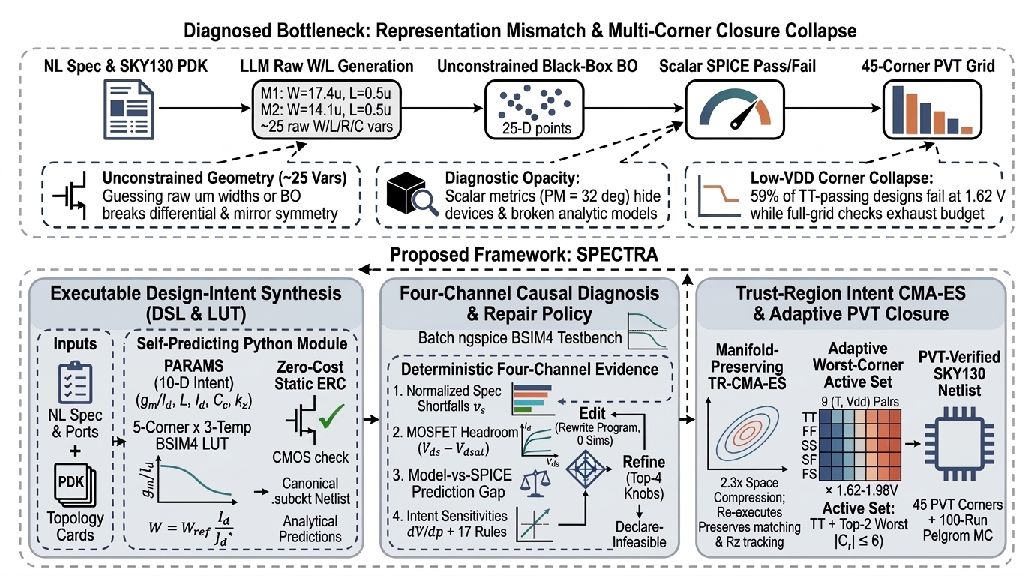
\includegraphics[width=0.98\textwidth]{figs/spectra_framework.pdf}
\vspace{-2.5mm}
\caption{Architecture of \textsc{SPECTRA}. Given a natural-language circuit specification and shared PDK/topology cards, \textbf{(a)} the LLM synthesizes an executable Python design-intent program that queries pre-characterized SKY130 BSIM4 lookup tables (\texttt{lut.size}) across 5 corners and 3 temperatures to emit both a canonical \texttt{.subckt} netlist and analytical self-predictions; \textbf{(b)} a static electrical-rule checker (ERC) filters illegal topologies at zero simulation cost before batch \texttt{ngspice} testbenches extract all target metrics; \textbf{(c)} a four-channel causal analyzer extracts normalized violations, device operating-region margins ($V_{DS}-V_{dsat}$), prediction-to-simulation discrepancies, and finite-difference intent sensitivities to steer a hierarchical policy (\textsc{Edit}, \textsc{Refine}, or \textsc{Declare-Infeasible}); and \textbf{(d)} bounded trust-region CMA-ES searches the low-dimensional intent space while preserving matching and bias invariants, closing 45-condition PVT targets via adaptive worst-corner promotion.}
\Description{System architecture diagram of SPECTRA showing four connected stages: executable design-intent program synthesis with BSIM4 lookup tables, static ERC and ngspice testbench evaluation, four-channel device-level causal diagnosis with hierarchical repair routing, and trust-region intent-space CMA-ES with adaptive 45-corner PVT verification.}
\label{fig:overview}
\end{figure*}


\subsection{Problem Definition and Framework Overview}
\label{sec:formulation}
We consider an analog synthesis task $\mathcal{T} = (x_{\text{NL}}, \mathcal{P}_{\text{io}}, \mathcal{B}, \mathcal{S}, \mathcal{C}_{\text{eval}})$, where $x_{\text{NL}}$ is a natural-language specification, $\mathcal{P}_{\text{io}}$ defines the subcircuit port interface, $\mathcal{B}$ is a family-specific SPICE testbench suite, $\mathcal{S} = \{(s, \circ_s, \tau_s)\}_{s=1}^{|\mathcal{S}|}$ specifies quantitative performance targets with comparator $\circ_s \in \{\ge, \le, \text{range}\}$ and threshold $\tau_s$, and $\mathcal{C}_{\text{eval}}$ denotes the verification condition set. Nominal tasks evaluate $\mathcal{C}_{\text{eval}} = \{c_{\text{TT}}\}$ at $(27\,^\circ\mathrm{C}, V_{DD}=1.8\,\mathrm{V})$, whereas robust tasks require simultaneous satisfaction across $|\mathcal{C}_{\text{PVT}}| = 45$ corners spanning $\{\text{TT, FF, SS, SF, FS}\} \times \{-40, 27, 125\,^\circ\mathrm{C}\} \times \{1.62, 1.80, 1.98\,\mathrm{V}\}$. Given $\mathcal{T}$, the synthesizer must emit a transistor-level SKY130 subcircuit netlist $N^*$ built exclusively from physical foundry primitives ($1.8\,\mathrm{V}$ BSIM4 nFET/pFET devices, vertical substrate PNPs, temperature-modeled high-resistance poly resistors, and MIM capacitors, with zero ideal internal sources) satisfying all constraints in $\mathcal{S}$ across $\mathcal{C}_{\text{eval}}$ within hard budgets of $B_{\text{LLM}}$ LLM calls and $B_{\text{sim}}$ SPICE condition-evaluations.

Figure~\ref{fig:overview} depicts the architecture of \textsc{SPECTRA}. Rather than prompting the LLM to emit raw transistor widths, \textsc{SPECTRA} organizes closed-loop synthesis into three core modules coupled to a multi-corner optimization protocol: \textbf{(1) Executable Design-Intent Synthesis} (Section~\ref{sec:intent}), which compiles low-dimensional Python $g_m/I_D$ programs through BSIM4 lookup tables and zero-cost static electrical-rule checking (ERC) into canonical netlists and analytical self-predictions; \textbf{(2) Four-Channel Causal Diagnosis} (Section~\ref{sec:diag}), which converts SPICE operating points, prediction discrepancies, and parameter sensitivities into physical root-cause evidence; and \textbf{(3) Hierarchical Repair and Trust-Region Intent Refinement} (Section~\ref{sec:refine}), which routes between symbolic program edits and symmetry-preserving CMA-ES under the minimax multi-corner objective and adaptive PVT schedule in Section~\ref{sec:opt}.

\subsection{Executable Design-Intent Synthesis}
\label{sec:intent}
\begin{figure}[t]
\begin{lstlisting}[style=prog]
PARAMS = {"gmid1": (18, 14, 22), "L1": (1.0, .5, 2),  # intent
  "It": (30e-6, 15e-6, 60e-6), "I7": (120e-6, 60e-6, 250e-6),
  "gmidp": (10, 7, 13), "Lp": (.8, .4, 1.5), "Cc": (1e-12, .5e-12, 2e-12),
  "gmidn": (13, 9, 16), "Ln": (2, 1, 3), "kRz": (1.6, .8, 3.5)}
def design(p, lut, spec):
  m1 = lut.size("n", p["gmid1"], p["L1"], p["It"]/2, vds=.5, vsb=.25)
  m3 = lut.size("p", p["gmidp"], p["Lp"], p["It"]/2, vds=.75)
  m7 = lut.size("p", p["gmidp"], p["Lp"], p["I7"], vds=.9)
  ...                                    # tail, bias, M8
  n = Netlist("vinp vinn vout vdd vss ibias")
  n.dev("M1", "d1", "vinn", "tail", "vss", m1)
  n.dev("M7", "vout", "o1", "vdd", "vdd", m7)       # ...
  n.R("RZ", "o1", "cz", p["kRz"] / m7.gm)
  A = m1.gm/(m1.gds+m3.gds) * m7.gm/(m7.gds+m8.gds)
  ugbw = m1.gm / (2*PI*p["Cc"])
  return n, {"gain_db": db(A), "ugbw": ugbw, "pm": ..., ...}
\end{lstlisting}
\vspace{-2mm}
\caption{Excerpt of a design-intent program written by SPECTRA for a two-stage op-amp task (abridged). Sizes come
from $(g_m/I_D, L, I_D)$ through \texttt{lut.size}; the returned predictions are compared against simulation.}
\label{fig:program}
\end{figure}


An executable design-intent program (Figure~\ref{fig:program}) is a sandboxed Python module declaring a bounded parameter dictionary \texttt{PARAMS} and a deterministic sizing function \texttt{design(p, lut, spec)}. \texttt{PARAMS} specifies $d$ continuous physical intent knobs $p = (p_1, \dots, p_d)$ with initial values and box bounds $[\ell_i, u_i]$, typically spanning $3 \le d \le 12$ degrees of freedom such as transconductance efficiencies $(g_m/I_D)$, channel lengths $L$, branch currents $I_D$, compensation capacitances $C_c$, and zero-nulling ratios $k_z$. Inside \texttt{design}, device dimensions are resolved not by guessing widths, but by querying pre-characterized SKY130 BSIM4 lookup tables~\cite{jespers2017gmid} tabulated over $\{5\text{ corners}\} \times \{-40, 27, 125\,^\circ\mathrm{C}\}$ on an $11 \times 10 \times 5 \times 181$ $(L, V_{DS}, V_{SB}, V_{GS})$ grid at reference finger width $W_{\text{ref}} = 5\,\mu\mathrm{m}$. Given $(g_m/I_D, L, I_D, V_{DS}, V_{SB})$, \texttt{lut.size} performs trilinear interpolation in $(\log L, V_{DS}, V_{SB})$, inverts $(g_m/I_D)(V_{GS})$ along the monotone moderate-to-strong inversion branch to obtain normalized current density $J_D^* = I_D / W_{\text{ref}}$, and computes device width deterministically:
\begin{equation}
  W = W_{\text{ref}} \cdot \frac{I_D}{J_D^*\!\big(g_m/I_D,\, L,\, V_{DS},\, V_{SB}\big)},
  \label{eq:lut_size}
\end{equation}
returning $(W, V_{GS}, V_{th}, V_{dsat}, g_m, g_{ds}, C_{gg}, C_{gd}, f_T)$ while partitioning $W$ into parallel fingers of width at most $5\,\mu\mathrm{m}$ to suppress narrow/wide geometry drift. Cross-corner queries \texttt{lut.at(corner, T)} further expose corner shifts analytically. Before invoking SPICE, a canonical parser and static ERC validate port signatures, DC supply/ground paths (eliminating floating gates), legal bulk ties (p-substrate nFET bodies and grounded PNP collectors), and PDK geometry bounds at zero simulation cost.

Crucially, \texttt{design} returns both the compiled netlist $N(p)$ and analytical self-predictions $\hat{m}(p)$ for every constrained specification. Comparing $\hat{m}_s(p)$ against simulated $m_{s,c}(N(p))$ directly isolates flaws in the LLM's symbolic circuit equations (such as omitting cascode output conductance or fold-branch slew limits), providing a structural signal unavailable from raw metric pass/fail logs.

\subsection{Four-Channel Causal Diagnosis}
\label{sec:diag}
For each constraint $s \in \mathcal{S}$ and condition $c$, we define a dimensionless shortfall $v_s(m_{s,c}) \ge 0$ ($v_s = 0$ iff satisfied): for positive scale-invariant quantities (bandwidth, power, slew, settling, noise, regulation), $v_s(m) = \max(0, \log_{10}(\tau_s / m))$ when $\circ_s$ is $\ge$ (and $\log_{10}(m / \tau_s)$ when $\le$); for linear or decibel targets, $v_s(m) = \max(0, (\tau_s - m)/|\tau_s|)$ (or $(m - \tau_s)/|\tau_s|$); and for interval targets $[\tau_{\text{lo}}, \tau_{\text{hi}}]$, out-of-range distance normalized by $(\tau_{\text{hi}} - \tau_{\text{lo}})$.

Whenever verification fails, \textsc{SPECTRA}'s deterministic analyzer synthesizes four structured evidence channels:
(1) a \emph{specification shortfall table} contrasting target $\tau_s$, SPICE value $m_{s,c}$, analytical prediction $\hat{m}_s$, and shortfall $v_s$;
(2) a \emph{MOSFET operating-region headroom map} classifying every transistor into saturation ($V_{DS} - V_{dsat} \ge 50\,\mathrm{mV}$), edge-of-saturation ($0 \le V_{DS} - V_{dsat} < 50\,\mathrm{mV}$), triode ($V_{DS} < V_{dsat}$), subthreshold ($V_{GS} < V_{th} - 50\,\mathrm{mV}$), or cutoff ($I_D < 1\,\mathrm{nA}$), annotated with $I_D$, $g_m/I_D$, $g_m/g_{ds}$, and $V_{DS} - V_{dsat}$;
(3) \emph{model-mismatch alerts} flagging metrics where $|\hat{m}_s / m_{s,c} - 1| > 0.25$ ($>6\,\mathrm{dB}$ for gain/rejection or $>10^\circ$ for phase margin); and
(4) \emph{finite-difference intent sensitivities}, evaluated near feasibility ($\mathcal{V} < 4$) by perturbing up to eight intent knobs by $+10\%$ (debited from $B_{\text{sim}}$) to obtain directional violation derivatives $\Delta_i \mathcal{V} = \mathcal{V}(p + 0.1 p_i e_i) - \mathcal{V}(p)$.
On nominal tasks with valid derivatives, a 1-simulation bounded coordinate step tests the top four attributed knobs and retains the update strictly if SPICE violation decreases. Finally, 17 deterministic domain rules (4 device-region rules and 13 circuit-family rules) connect flagged devices to violated specifications, such as linking a triode tail sink to collapsed CMRR or rail-pinned DC output to stage current imbalance.

\subsection{Hierarchical Repair and Trust-Region Intent Refinement}
\label{sec:refine}
Conditioned on the current program, the four-channel diagnosis, retrieved family topology cards, and a rolling six-step trace, the LLM selects one of three repair actions:
(1) \textsc{Edit}, rewriting circuit topology, biasing architecture, or sizing equations in Python (1 LLM call, 0 optimization simulations);
(2) \textsc{Refine}, retaining the symbolic program while optionally updating parameter bounds and invoking continuous intent search (0 LLM calls); or
(3) \textsc{Declare-Infeasible}, terminating with a physical trade-off rationale.

Under \textsc{Refine}, active parameters $p_i \in [\ell_i, u_i]$ are normalized to unit coordinates $u_i \in [0, 1]$ (logarithmically when $\ell_i > 0$ and $u_i / \ell_i > 4$, linearly otherwise). When sensitivity attribution yields nonzero violation derivatives, optimization concentrates on the top $d_{\text{act}} \le 4$ active knobs; otherwise all $d$ intent parameters are searched. Around incumbent $u^{(0)}$ at refinement round $t$, \textsc{SPECTRA} forms an expanding box trust region $[\max(0, u^{(0)} - r_t), \min(1, u^{(0)} + r_t)]$ with radius $r_t = \min(0.25, 0.08 + 0.02 t)$, runs coordinate boundary probes at $\pm r_t$, and executes covariance matrix adaptation evolution strategy (CMA-ES)~\cite{hansen2016cma} with step size $\sigma_0 = \min(0.15, r_t/2)$ and population $\lambda = \max(8, 4 + \lfloor 3 \ln d_{\text{act}} \rfloor)$. Every candidate $u$ re-executes \texttt{design(p(u), lut, spec)}, guaranteeing that differential-pair symmetry, mirror ratios, and tracking passives ($R_z = k_z / g_{m7}$) hold identically along the entire optimization trajectory.

\subsection{Optimization Objective, Adaptive PVT Closure, and Execution Protocol}
\label{sec:opt}
Both directional probes and trust-region CMA-ES are supervised directly by batch SPICE measurements through the capped minimax multi-corner violation objective over active condition set $\mathcal{C}$:
\begin{equation}
  \mathcal{V}_{\mathcal{C}}(p) = \max_{c \in \mathcal{C}} \sum_{s \in \mathcal{S}} \min\!\Big(2,\, v_s\!\big(m_{s,c}(N(p))\big)\Big),
  \label{eq:viol}
\end{equation}
where capping individual metric shortfalls at $2$ prevents a single unconverged or rail-pinned metric from dominating rank-based covariance updates across remaining specifications.

\textbf{Adaptive Worst-Corner PVT Closure.} Evaluating all 45 corners per CMA-ES candidate would multiply inner-loop SPICE cost by $45\times$. On robust tasks, \textsc{SPECTRA} first closes nominal targets on $\mathcal{C}_0 = \{c_{\text{TT}}\}$ and performs one 45-corner verification sweep. If $\mathcal{V}_{\mathcal{C}_{\text{PVT}}}(p) = 0$, synthesis succeeds immediately. Otherwise, \textsc{SPECTRA} seeds an active corner set $\mathcal{C}_1 = \{c_{\text{TT}}\} \cup \operatorname{Top-2}(\mathcal{C}_{\text{PVT}})$ with the two worst-violating corners, minimizes Eq.~\eqref{eq:viol} over $\mathcal{C}_1$, re-verifies on $\mathcal{C}_{\text{PVT}}$, and promotes up to two newly worst corners per round:
\begin{equation}
  \mathcal{C}_{r+1} = \mathcal{C}_r \,\cup\, \operatorname*{Top-2}_{c \in \mathcal{C}_{\text{PVT}} \setminus \mathcal{C}_r} \mathcal{V}_{\{c\}}(p^{(r)}), \quad |\mathcal{C}_{r+1}| \le 6,
  \label{eq:active_set}
\end{equation}
for up to three rounds before returning persistent corner violations to the LLM for structural headroom redesign.

\textbf{Training-Free Execution and Test-Time Verification.} \textsc{SPECTRA} operates strictly zero-shot with frozen LLM weights and zero reference circuits in prompts or topology cards. During test-time synthesis, every SPICE run (nominal checks, finite-difference sensitivities, trust-region CMA-ES populations, and 45-corner sweeps) is strictly charged against $B_{\text{sim}}$. Upon termination, an independent out-of-loop verifier re-simulates the emitted `.subckt` netlist across all $c \in \mathcal{C}_{\text{eval}}$, supplemented by 100-sample Pelgrom mismatch Monte Carlo on PVT-verified designs.
